\clearpage
\chapter{和声进阶：七和弦、声部进行与再配和}
\label{chap:advanced-harmony}

\subsection*{学完这一章能做什么}
\begin{itemize}
  \item 分清属七、大七、小七、半减七、减七的构成与功能位置，不再把“七和弦”当成一种颜色。
  \item 用共同音、级进与解决三原则检查四声部进行，能指出平行五度/八度与未解决七音。
  \item 用转位、drop-2、持续低音与模进式再配和给同一段旋律做三个版本。
  \item 在夜半里把八小节 I--vi--IV--V 改成 ii--V--I 与借用和弦版本，比较低音线与紧张度。
\end{itemize}

\subsection{七和弦的五种性质}

七和弦 = 三和弦 + 七音。性质由“三音、五音、七音”各自与根音的音程决定：

\begin{center}
\small
\begin{tabular}{clll}
\toprule
性质 & 构成（半音） & 记号 & 常见位置 \\
\midrule
属七 & 4, 7, 10 & X7 & V7，蓝调 I7/IV7 \\
大七 & 4, 7, 11 & Xmaj7 & Imaj7、IVmaj7 \\
小七 & 3, 7, 10 & Xm7 & ii7、vi7、iii7 \\
半减七 & 3, 6, 10 & Xm7\(\flat\)5 & viiø7、iiø7（小调） \\
减七 & 3, 6, 9 & Xdim7 & 经过/对称张力，少作稳定主和弦 \\
\bottomrule
\end{tabular}
\end{center}

功能写作里最常用的是 ii7--V7--Imaj7：ii7 的小七度里含主音的六度，V7 的三全音（3 与 \(\flat\)7）指向 I，Imaj7 的大七度把“到家”钉住。不要把 V7 的 \(\flat\)7 当成装饰：它必须下行级进到 I 的三音，否则听感会“悬着”。

\subsection{声部进行：三条硬规则与两条软规则}

四声部写作（SATB 或四部器乐）先看横向，再看纵向。硬规则：

\begin{enumerate}
  \item \textbf{解决七音}：V7 的七音下行级进到 I 的三音；ii7 的七音下行到 V7 的三音。
  \item \textbf{解决导音}：V7 的三音（大调导音）上行到 I 的主音；若在内声部可下行到五音，但不能跳进。
  \item \textbf{不做平行五度/八度}：两个声部从纯五度/八度同向走到另一个纯五度/八度，会削弱独立声部感。
\end{enumerate}

软规则：

\begin{itemize}
  \item 优先共同音，其次级进，最后才用跳进；跳进后反向级进补偿。
  \item 低音与旋律反向进行，外声部不要同时大跳。
  \item 和弦音重复优先根音与五音；三音（导音）与七音尽量不重复。
\end{itemize}

\begin{figure}[htbp]
\centering
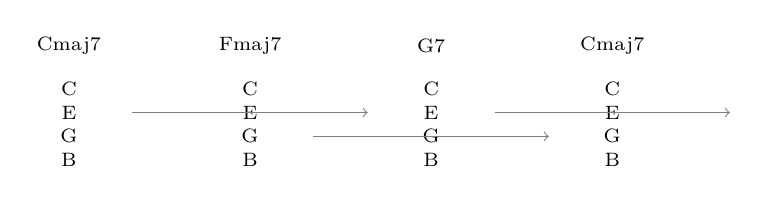
\begin{tikzpicture}[x=2.3cm,y=0.55cm,font=\scriptsize]
  \foreach \x/\ch/\n in {0/Cmaj7/{C E G B},1/Fmaj7/{F A C E},2/G7/{G B D F},3/Cmaj7/{C E G B}} {
    \node at (\x,2.6) {\ch};
    \foreach \i/\t in {0/C,1/E,2/G,3/B} { \node at (\x,1.6-\i*0.55) {\t}; }
  }
  \draw[->,gray] (0.35,1.05)--(1.65,1.05);
  \draw[->,gray] (1.35,0.5)--(2.65,0.5);
  \draw[->,gray] (2.35,1.05)--(3.65,1.05);
\end{tikzpicture}
\caption*{图 11-1：Cmaj7--Fmaj7--G7--Cmaj7 的共同音与级进。共同音尽量保留，其余声部走最小步；G7 的 F 下行到 Cmaj7 的 E，B 上行到 C。}
\end{figure}

\subsection{转位、drop-2 与低音线}

转位（inversion）把和弦的低音换成三音、五音或七音，改变的是低音线，不是和弦性质。写作时先定低音线，再选转位：

\begin{itemize}
  \item \textbf{第一转位}：三音在低音，适合让低音级进（C--E--G--B 的低音可走 C--E--G--B）。
  \item \textbf{第二转位}：五音在低音，常作经过或持续低音上的和弦。
  \item \textbf{drop-2}：把四声部中第二高的音下移八度，得到更开阔的键盘/吉他排列；注意下移后不要与低音撞在一起。
\end{itemize}

例：C--F--G--C 的低音线若写成 C--F--G--C 会四度跳；改成 C--F/A--G/B--C，低音走 C--A--B--C，级进更平滑，但 F/A 的第二转位要避免长期停留。

\subsection{再配和：同一旋律的三种做法}

再配和（reharmonisation）不是“换一堆奇怪和弦”，而是改变和声对旋律的解释。三种可控手法：

\begin{enumerate}
  \item \textbf{功能替换}：I 可换 vi 或 iii；IV 可换 ii；V 可换 viiø7 或替代属和弦。前提是低音与旋律仍能听成同一功能。
  \item \textbf{持续低音}：低音固定，和弦在上层变化，制造“同一根、不同颜色”；适合前奏/桥段。
  \item \textbf{模进式再配和}：把同一动机的和声整体下移/上移二度或三度，保持声部关系；模进超过两次要回收，否则会变成练习曲。
\end{enumerate}

\begin{center}
\small
\begin{tabular}{clll}
\toprule
原进行 & 替换 & 听感 & 风险 \\
\midrule
I--vi--IV--V & ii--V--I--vi & 更爵士、低音下行 & ii7 的七音要解决 \\
I--IV--V--I & I--IV--ii--V & 更平滑、延迟到主 & ii 与 V 的七音链要算清 \\
I--V--vi--IV & I--V--vi--IV（借用 Fm） & 更暗、副歌前对比 & Fm 后要能回 C \\
\bottomrule
\end{tabular}
\end{center}

在夜半里做：把八小节分成两半，前半 I--vi--IV--V，后半 ii--V--I--V；把每小节低音单独抽出来听，如果低音跳超过四度，先用转位修低音，再谈颜色。

\subsection{练习}
\begin{enumerate}
  \item 写出 C 大调 V7 的四个音，并说明七音与三音各解决到哪个音。\\
  \emph{答案：}G B D F；F 下行到 E，B 上行到 C。
  \item 为什么 V7 的三音在内声部可以下行，而导音在外声部通常上行？\\
  \emph{答案：}外声部导音的指向性最强；内声部下行到五音可避免声部交叉，但仍不能跳进。
  \item 给 C--F--G--C 写一条级进低音线，标出所用转位。\\
  \emph{答案示例：}C--F/A--G/B--C；F 第一转位、G 第一转位。
  \item 把 I--vi--IV--V 改成 ii--V--I--vi，指出哪个七音必须解决。\\
  \emph{答案：}ii7 的七音下行到 V7 的三音；V7 的七音再下行到 I 的三音。
  \item 用持续低音给 C 大调旋律配四小节，写出上层和弦。\\
  \emph{答案示例：}低音 C 持续，上层 Cmaj7--Fmaj7/C--Dm7/C--G7/C。
  \item 在夜半里铺八小节 I--vi--IV--V，把低音改成 C--A--F--G，再把前半改成 ii--V--I--vi，比较两次低音线的跳进与七音解决。\\
  \emph{答案示例：}原版低音 C--A--F--G 有三度/四度跳；改版 C--D--C--A 更级进，但 ii7 的七音要下行到 V7 的三音，不能停在小节线上。
\end{enumerate}

\subsection{帮助主题映射}
\begin{center}
\footnotesize
\setlength{\tabcolsep}{3pt}
\begin{longtable}{p{0.34\linewidth}p{0.45\linewidth}p{0.15\linewidth}}
\toprule
本章小节 & 应用内帮助锚点 & 备注 \\
\midrule
\endhead
七和弦性质 & \texttt{music-theory-seventh-chords} & 表 11-1 \\
声部进行规则 & \texttt{music-theory-voice-leading} & 图 11-1 \\
转位与低音线 & \texttt{music-theory-inversions-bass} & 操作 \\
再配和三法 & \texttt{music-theory-reharmonisation} & 表 11-2 \\
在夜半里怎么做 & \texttt{music-theory-reharmonise-eight-bars} & 操作 \\
练习 & \texttt{music-theory-ch11-practice} & 答案在本章 \\
\bottomrule
\end{longtable}
\end{center}
